% lonlat.tex

\subsection{Système de coordonnées}

Un point $\mathbf{x}$ de la sphère $ \mathbb{S}_a^2 = \{ (x,y,z) \in \mathbb{R}^3 \text{ tel que } x^2 + y^2 + z^2 = a^2\}$ est repéré par ses coordonnées longitude-latitude $(\lambda, \theta ) \in ]0, 2\pi ] \times ]- \pi/2, \pi/2 [$. La donnée $\lambda$ est la longitude du point donnée par l'angle équatorial et $\theta$ est l'angle latitudinal (Voir Fig. \ref{fig:lonlat_sphere}). Il peut aussi être repéré par ses coordonnées cartésiennes $(x,y,z) \in \mathbb{R}^3$.

\begin{figure}
\begin{center}
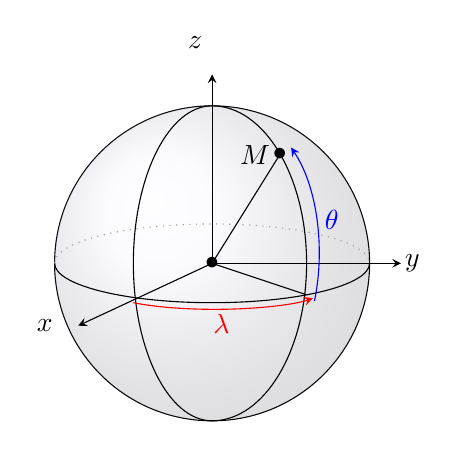
\begin{tikzpicture}[scale=2]
\draw (0,0) circle (1) ;
\shade[ball color=blue!10!white,opacity=0.20] (0,0) circle (1);
\draw (-1,0) arc (180:360:1cm and 0.25cm);

\draw (-1,0)[dotted, color=black!40] arc (180:360:1cm and -0.25cm);
\draw (0,1) arc (90:270:0.5cm and 1cm);
\draw (0,1) arc (90:-90:0.6cm and 1cm);

\draw (0,0) node {$\bullet$} ;

\draw [>=stealth, ->] (0,0) -- (-0.85,-0.396) ;
\draw (-0.95,-0.396) node[left]{$x$} ;   
\draw [>=stealth, ->] (0,0) -- (1.2,0) ;
\draw (1.38,0) node[left]{$y$} ;   
\draw [>=stealth, ->] (0,0) -- (0,1.2) ;
\draw (0,1.4) node[left]{$z$} ;   

\draw (0,0) -- (0.6,-0.2) ;
\draw (0,0) -- (0.43,0.69) ;
\draw (0.43,0.69) node {$\bullet$} ;
\draw (0.43,0.69) node[left]{$M$} ;

\draw (-0.5,-0.25)[>=stealth, ->, color=red] arc (222.5:333:0.7cm and 0.13cm);
\draw (0.06,-0.26)[color=red] node[below]{$\lambda$} ;
\draw (0.65,-0.24)[>=stealth, ->, color=blue] arc (-20:50:0.5cm and 0.88cm);
\draw (0.76,0.4)[color=blue] node[below]{$\theta$} ;
\end{tikzpicture}
\end{center}
\caption{Longitude-Latitude}
\label{fig:lonlat_sphere}
\end{figure}


Les coordonnées cartésiennes $(x,y,z)$ et longitude-latitude $(\lambda, \theta)$ sont liées par :
\begin{equation}
\left\lbrace 
\begin{array}{rcl}
x & = & a \cos \theta \cos \lambda \\
y & = & a \cos \theta \sin \lambda \\
z & = & a \sin \theta.
\end{array}
\right.
\end{equation}
On construit la base associée sur la sphère. La base $( \mathbf{g}_{\lambda}, \mathbf{g}_{\theta})$ est donnée en $\mathbf{x} (x,y,z) \in \mathbb{S}_a^2$ par :
\begin{equation}
\mathbf{g}_{\lambda} = \dfrac{\partial \mathbf{x}}{\partial \lambda} = \begin{bmatrix}
- a \cos \theta \sin \lambda \\ 
a \cos \theta \cos \lambda \\ 
0
\end{bmatrix} 
\end{equation}
ainsi que 
\begin{equation}\label{coord_latlon}
\mathbf{g}_{\theta} = \dfrac{\partial \mathbf{x}}{\partial \theta} = \begin{bmatrix}
- a \sin \theta \cos \lambda \\ 
- a \sin \theta \sin \lambda \ \\ 
a \cos \theta.
\end{bmatrix} 
\end{equation}

\begin{remarque}
\label{base_lonlat}
On normalise cette base en $\mathbf{e}_{\lambda} = \dfrac{1}{\| \mathbf{g}_{\lambda} \|} \mathbf{g}_{\lambda}$ et $\mathbf{e}_{\theta} = \dfrac{1}{\| \mathbf{g}_{\theta} \|} \mathbf{g}_{\theta}$. Si $\mathbf{F} \in \mathbb{T}\mathbb{S}_a$ alors il existe $F_{\lambda}$ et $F_{\theta}$ tels que $\mathbf{F} = F_{\lambda} \mathbf{e}_{\lambda} + F_{\theta} \mathbf{e}_{\theta}$.
\end{remarque}

Ainsi la métrique $\mathbf{G}$ est :
\begin{equation}
\mathbf{G} = 
\begin{bmatrix}
\mathbf{g}_{\lambda} \cdot \mathbf{g}_{\lambda} & \mathbf{g}_{\lambda} \cdot \mathbf{g}_{\theta} \\
\mathbf{g}_{\theta} \cdot \mathbf{g}_{\lambda} & \mathbf{g}_{\theta} \cdot \mathbf{g}_{\theta}
\end{bmatrix}
 =
\begin{bmatrix}
a^2 \cos \theta & 0 \\
0 & a^2
\end{bmatrix}
\end{equation}

On pose $\overline{\mathbf{G}} = det (\mathbf{G}) = a^4 \cos^2 \theta$. La base $( \mathbf{g}^{\lambda}, \mathbf{g}^{\theta} )$ est telle que :

\begin{equation}
\left\lbrace 
\begin{array}{rcl}
\mathbf{g}^{\lambda} & = & \mathbf{G}^{1,1} \mathbf{g}_{\lambda} + \mathbf{G}^{1,2} \mathbf{g}_{\theta} \\
\mathbf{g}^{\theta} & = & \mathbf{G}^{2,1} \mathbf{g}_{\lambda} + \mathbf{G}^{2,2} \mathbf{g}_{\theta}, \\
\end{array}
\right.
\end{equation}
avec $\mathbf{G}^{i,j} = \left( \mathbf{G}^{-1} \right)_{i,j}$.
De là, il découle :
\begin{eqsys}
\mathbf{g}^{\lambda} = \dfrac{1}{a \cos \theta}  \mathbf{e}_{\lambda} \\
\mathbf{g}^{\theta} = \dfrac{1}{a} \mathbf{e}_{\theta}.
\end{eqsys}
A partir de ces vecteurs élémentaires, on peut obtenir des formules pour calculer les opérateurs différentiels classiques sur la sphère ainsi que l'intégrale sur la surface d'une sphère.

\subsection{Opérateurs classiques sur la sphère}

Soit une fonction $h: \mathbf{x} \in \mathbb{S}_a^2 \mapsto h(\mathbf{x})$ régulière. On peut calculer le gradient de $h$ par :
\begin{equation}
\nabla_T h = \dfrac{\partial h}{\partial \lambda} \mathbf{g}^{\lambda} + \dfrac{\partial h}{\partial \theta} \mathbf{g}^{\theta}
\end{equation}
ce qui se traduit en :
\begin{equation}\label{gradient_lonlat}
\nabla_T h = \dfrac{1}{a \cos \theta}\dfrac{\partial h}{\partial \lambda} \mathbf{e}_{\lambda} + \dfrac{1}{a} \dfrac{\partial h}{\partial \theta} \mathbf{e}_{\theta}.
\end{equation}
Soit un champ de vecteurs sur la sphère $\mathbf{F} = F_{\lambda} \mathbf{e}_{\lambda} + F_{\theta} \mathbf{e}_{\theta}$ régulier. Alors 
\begin{eqsys}
\mathbf{F} \cdot \mathbf{g^{\lambda}} = \dfrac{1}{a \cos \theta} F_{\lambda} \\
\mathbf{F} \cdot \mathbf{g^{\theta}} = \dfrac{1}{a} F_{\theta}.
\end{eqsys}
La divergence de $\mathbf{F}$ est donnée par :
\begin{equation}
\nabla_T \cdot \mathbf{F} = \dfrac{1}{\sqrt{\overline{\mathbf{G}}}} \left( \dfrac{\partial}{\partial \lambda} \left( \sqrt{\overline{\mathbf{G}}} \mathbf{F} \cdot \mathbf{g}^{\lambda}  \right) +  \dfrac{\partial}{\partial \theta} \left( \sqrt{\overline{\mathbf{G}}} \mathbf{F} \cdot \mathbf{g}^{\theta}  \right)  \right)
\end{equation}
d'où :
\begin{equation}\label{divergence_lonlat}
\nabla_T \cdot \mathbf{F} = \dfrac{1}{a \cos \theta} \dfrac{\partial}{\partial \lambda}  F_{\lambda} + \dfrac{1}{a \cos \theta} \dfrac{\partial}{\partial \theta} \left( \cos \theta F_{\theta} \right).
\end{equation}
Le rotationnel de $\mathbf{F}$ se calcule grâce au produit vectoriel. Il est donné par :
\begin{equation}
\nabla_T \wedge \mathbf{F} = \mathbf{g}^{\lambda} \wedge \dfrac{\partial}{\partial \lambda}\mathbf{F} + \mathbf{g}^{\theta} \wedge \dfrac{\partial}{\partial \theta}\mathbf{F}.
\end{equation}
Après calculs, on obtient :
\begin{equation}\label{rotationnel_lonlat}
\nabla_T \wedge \mathbf{F} = \left[ F_{\lambda} \dfrac{\tan \theta}{a} + \dfrac{1}{a \cos \theta} \dfrac{\partial F_{\theta}}{\partial \lambda} - \dfrac{1}{a} \dfrac{\partial F_{\lambda}}{\partial \theta} \right] \mathbf{e}_R - \dfrac{F_{\theta}}{a} \mathbf{e}_{\lambda},
\end{equation}
avec $\mathbf{e}_{R} = \left( \cos \theta \cos \lambda, \cos \theta \sin \lambda, \sin \theta \right)^T$. Le Laplacien est la composition des deux opérateurs précédents : $\Delta_T h = \nabla_T \cdot \nabla_T h$ :
\begin{equation}\label{laplacien_lonlat}
\Delta_T h = \dfrac{1}{a^2 \cos^2 \theta} \dfrac{\partial^2 h }{\partial \lambda^2} + \dfrac{1}{a^2 \cos \theta} \dfrac{\partial}{\partial \theta} \left( \cos \theta \dfrac{\partial h}{\partial \theta} \right).
\end{equation}
En plus des opérateurs différentiels courants, en utilisant le changement de variable $\mathbf{x} \mapsto (\lambda, \theta)$ issu de \eqref{coord_latlon}, on peut donner une formule d'intégration :
\begin{equation}\label{integrale_lonlat}
\gint_{\mathbb{S}_a^2} h(\mathbf{x})d\sigma(\mathbf{x})= \gint_{\lambda=0}^{2 \pi} \gint_{\theta = - \pi/2}^{\pi/2} h(\lambda, \theta) \underbrace{a^2 \cos \theta}_{\sqrt{\overline{\mathbf{G}}}} d \theta d \lambda.
\end{equation}
